\documentclass{beamer}
%
% Choose how your presentation looks.
%
% For more themes, color themes and font themes, see:
% http://deic.uab.es/~iblanes/beamer_gallery/index_by_theme.html
%
\mode<presentation>
{
	\usetheme{default}      % or try Darmstadt, Madrid, Warsaw, ...
	\usecolortheme{default} % or try albatross, beaver, crane, ...
	\usefonttheme{default}  % or try serif, structurebold, ...
	\setbeamertemplate{navigation symbols}{}
	\setbeamertemplate{caption}[numbered]
	\setbeamertemplate{footline}{%
		\raisebox{5pt}{\makebox[\paperwidth]{\hfill\makebox[10pt]{\scriptsize\insertframenumber}}}}
	\setbeamertemplate{bibliography item}{\insertbiblabel}
} 

\usepackage{ngerman}
\usepackage{graphicx}
\usepackage[latin1]{inputenc}
\usepackage{amscd}
\usepackage{amssymb}
\usepackage{amsmath}
\usepackage{bibgerm}
\usepackage{nameref}

\usepackage{lipsum}

\newcommand\blfootnote[1]{%
	\begingroup
	\renewcommand\thefootnote{}\footnote{#1}%
	\addtocounter{footnote}{-1}%
	\endgroup
}
\usepackage{pdfcomment}
\newcommand{\pdfnote}[1]{\marginnote{\pdfcomment[icon=note]{#1}}}

\title{Rigging - Skinning - Rendering}
\author{Marcel Gross, Julian Kurz, Christian Braun}
\institute{Schwerpunktseminar Medieninformatik Fachhochschule Wuerzburg-Schweinfurt}
\date{\today}

\bibliographystyle{geralpha}

\begin{document}
	
	\begin{frame}
		\titlepage
	\end{frame}
	
	
	\begin{frame}{}
		\tableofcontents
	\end{frame}
	
	\newpage
\section{Rigging}
\label{sec:whats_rigging}
Rigging ist ein Teil der Computeranimation, wobei die Skelettanimation eines der am h�ufigsten genutzten Methoden ist. Bei dieser Methode wird ein hierarchisch aufgebautes Skelett, ein 3D-Modell, welches im weiteren Verlauf als Mesh bezeichnet wird, und die Bewegungsdaten einzelner Punkte des Skeletts ben�tigt. Diese markanten Punkte, k�nnen zum Beispiel die Gelenke oder das Ende eines Fingers sein. Der Begriff Bewegungsdaten steht hier als Synonym f�r die 3D-Koordinaten im zeitlichen Verlauf einer Bewegung. Diese Koordinaten repr�sentieren einzelne Marker welche mit einem Motion Capturing System aufgenommen wurden.

Beim Rigging wird nun das Skelett mit dem Mesh verbunden. Die Verformung des Mesh w�hrend einer Bewegung, ist Teil des Skinning-Prozesses.
Rigging l�sst sich in zwei Hauptbereiche einteilen:
\begin{itemize}
	\item Manuelles Rigging
	\item Automatisches Rigging
\end{itemize}
F�r das manuelle Rigging ben�tigt man spezielle 3D Modellierungs Software wie Maya oder Blender. Ein erfahrener Fachmann muss hierbei manuell das Skelett im Mesh platzieren.

Diese Ausarbeitung behandelt das Thema automatisches Rigging. Auch dieser Unterpunkt des Riggings l�sst sich weiter aufteilen:
\begin{itemize}
	\item \nameref{sec:skeleton-extraction}
	\item \nameref{sec:skeleton-embedding}
\end{itemize}
Es gibt auch Ans�tze, welche beide Methoden verbinden \cite{combination}. Im weiteren Verlauf wird jedoch nur auf \nameref{sec:skeleton-extraction} und \nameref{sec:skeleton-embedding} eingegangen.
Das Ziel des automatischen Riggings liegt darin, dass der Prozess vereinfacht und beschleunigt wird. Bisher war die Platzierung des Skellets im Mesh f�r Anf�nger schwierig. Der automatisierte Rigging-Vorgang wird oft an drei Kenngr��en bemessen:

\begin{itemize}
	\item Performanz: Der Vorgang sollte nicht l�nger dauern als das manuelle Rigging.
	\item Allgemeing�ltigkeit: Der Vorgang sollte nicht auf bestimmte Modelle, z. B. humanoide Formen, begrenzt sein.
	\item Selbstst�ndigkeit: Die ben�tigte Interaktion mit dem Benutzer sollte m�glichst gering sein.
\end{itemize}
In der nachfolgenden Ausarbeitung werden die einzelnen Verfahren mithilfe dieser drei Aspekten evaluiert.

Um die Verwechslungsgefahr zu minimieren werden noch folgende Begriffe eingef�hrt:
\begin{itemize}
	\item Animation-Skelett: Hierarchisches Skelett mit Knochen und Gelenken.
	\item Kurven-Skelett: Mittelachse eines Meshs.
\end{itemize}
\newpage


\subsection{Skelett-Extraktion}
\label{sec:skeleton-extraction}

Der Abschnitt �ber die Skelett-Extraktion st�tzt sich auf die Arbeit von J. Pan et al. \cite{extraction}.
F�r die Skelett-Extraktion wird kein Animation-Skelett im Voraus ben�tigt. Dieses wird aus dem Mesh extrahiert. F�r diese Extraktion werden die Mittelachsen einzelner Mesh-Segmente ben�tigt. Bei einer Hand zum Beispiel die Achsen der f�nf Finger, des Handtellers und des Armansatzes.

Um die Mittelachsen eines 3D-K�rpers zu bestimmen wird eine geometrische Form, die 3D-Silhouette, eingef�hrt. Eine 3D-Silhouette im Nachfolgenden auch nur als Silhouette bezeichnet, ist eine zweidimensionale Projektion des Meshs, wobei die Tiefeninformationen (Koordinate auf der Z-Achse) nicht verloren geht, sondern mit abgespeichert wird.

Wurde eine geeignete Projektion, wie in Abbschnitt \ref{sec:projection_detection} beschrieben, gefunden. Wird eine \nameref{sec:global_search} durchgef�hrt. Diese Suche findet alle Punkte des Meshs ohne darauf zu achten, ob diese verbunden sind. Sind alle Punkte gefunden, wird eine \nameref{sec:local_search} ausgef�hrt. Diese verbindet nun die Punkte und ber�cksichtigt deren Verbindung zum Mesh. Im Anschluss wird bei der \enquote{\nameref{sec:curve_skeleton_extraction}} die Mittelachsen bestimmt und das Kurven-Skelett extrahiert. In Abbildung \ref{extraction_fig1} a) kann man diese Mittelachse sehen (blaue Achse). Die rote und gelbe Linie repr�sentieren jeweils eine Projektion des Meshs.

Um dieses angen�herte Skelett f�r die Computer Animation nutzbar zu machen werden im letzten Schritt (Abschnitt: \ref{sec:animation_skeleton_creation}) noch die Gelenke eingef�gt und die Achsen begradigt.

\subsubsection{Projektionsfindung}
\label{sec:projection_detection}
Die optimale Projektion hat m�glichst wenig Verdeckung und das Maximum an Oberfl�che.

Mathematisch kann die Silhouette wie folgt beschrieben werden:
\begin{equation}
\label{3d_silhouette}
C = \{c_{i}(x,y,z) \vert c_{i}(x,y,z)\in V, c'_{i}(x,y) \in C', C' \subset P, x_{c_{i}} = x_{c'_{i}}, y_{c_{i}} = y_{c'_{i}} \}
\end{equation}
Symbol-Erl�uterung:
\begin{itemize}
	\item $C$: Menge der Punkte der Silhouette
	\item $V$: Menge der Punkte des Meshs
	\item $P$: Menge der Punkte der Projektion	
\end{itemize}

\subsubsection{Globale Suche und Lokale Suche}
\paragraph{Globale Suche}
\label{sec:global_search}
F�r die globale Suche muss zun�chst einmal der Punkt mit dem gr��ten Y-Wert aus der Menge $P$ bestimmt werden. Dieser Punkt ist unser Startpunkt. Wurde dieser Punkt ermittelt, werden nun alle Nachbarpunkte gesucht, welche in einem Radius $r$ liegen, wobei $r$ ein experimenteller Wert ist welcher dem maximalen euklidischen Abstand des Startpunktes ($P_{1}$) mit seinen Nachbarpunkten entspricht.

Zur mathematischen Bestimmung des Radius $r$ kann folgende Gleichung herangezogen werden:
\begin{equation}
\label{radius}
r= \max \Vert q_{i}(x,y,z) - q(x,y,z)\Vert
\end{equation}
$q(x,y,z)$ steht f�r den momentanen Punkt und $q_{i}(x,y,z)$ f�r einen der Nachbarpunkte.

Um den n�chsten Punkt bestimmen zu k�nnen nutzt man den Vektor $\overrightarrow{OX}$ mit dem Startpunkt als Ursprung und den Winkel von $-\pi$ bis $\pi$. Der Punkt, welcher mit dem kleinsten Winkel mit dem Vektor verbunden ist, ist der n�chste Punkt. Nun werden wieder alle Nachbarpunkte zu Punkt 2 ($P_{2}$), welche in $r$ liegen gesucht. Der Punkt mit dem gr��ten Winkel $\angle P_{1}P_{2}P_{3}$ ist der gesuchte Punkt.

Jetzt wird das Suchen nach Nachbarpunkten und das Bestimmen des Punktes mit dem gr��ten Winkel solange wiederholt, bis man wieder beim Startpunkt angekommen ist.

Durch den oben genannten Vorgang konnte die 2D-Silhouette $C'$ bestimmt werden.
Anschlie�end wird zu jedem Punkt $ c'_{i}(x,y) \in C' $ die jeweils gespeicherte Z-Koordinate hinzugef�gt. Dadurch entsteht die Menge der 3D-Punkte $ C'' = \{c''_{i}(x,y,z) \in C'', x_{c''} = x_{c'}, y_{c''} = y_{c'} \} $.

F�r ein bessers Verst�ndnis kann man sich auch den Artikel von R.A. Jarvis zum Thema zur Identifikation von convexen H�llen in einem endlichen Set von Punkten \cite{convex} anschauen. Der signifikante Unterschied zwischen den beiden Methoden ist jedoch folgender: in der oben genannten Methode ist die Suche auf den Radius $r$ begrenzt.

\paragraph{Lokale Suche}
\label{sec:local_search}
Abbildung \ref{extraction_fig1} (b) zeigt, wie die Lokale Suche abl�uft.
F�r die lokale Suche werden nun alle Punkte der Menge $C''_{i}$ miteinander verbunden. Um die Punkte miteinander zu verbinden, wird wie folgt vorgegangen: 

1. Der Punkt $c''_{i}(x,y,z)$ wird als Startpunkt $c_{i1}(x,y,z)$ definiert und es werden alle verbundenen Nachbarpunkte aus V gesucht.

2. Es wird der Punkt $c_{i2}(x,y,z)$ gesucht, welcher den gr��ten Winkel $\angle c_{i2}c''_{i}c_{ij}$ besitzt. $c_{ij}$ ist der Vorg�nger von $c''_{i}$

3. Ausgehend von $c_{i2}$ wird nun wieder der Punkt gesucht welcher den gr��ten Winkel $\angle c_{i3}c_{i2}c_{i1}$ besitzt.

4. Wiederhole Schritt 3 solange bis man wieder bei $c''_{i}(x,y,z)$ angekommen ist oder der Abstand zwischen $c_{ij}(x,y,z)$ und $c''_{i}(x,y,z)$ kleiner als der Radius $r$ ist der mit der Formel \ref{radius} bestimmt wurde.

\subsubsection{Skelett-Erzeugung}
\paragraph{Kurven-Skelett-Extraktion}
\label{sec:curve_skeleton_extraction}
Die in den oberen beiden Abschnitten gefunden Punktmenge wird nun herangezogen um mithilfe der Delaunay-Triangulation ein Dreiecksnetz zu erstellen \cite{delaunay}. Dieses kann man in Abbildung \ref{extraction_fig1} (c) sehen. Anhand dieser Dreiecke k�nnen nun an allen Kanten, welche nicht die Au�enfl�chen des Meshs ber�hren, Mittelpunktbestimmungen vorgenommen werden. Daf�r wird berechnet: $ \vec{m_{k}} = \left( \frac{x_{i} + x_{j}}{2},\frac{y_{i} + y_{j}}{2},\frac{z_{i} + z_{j}}{2} \right)  $. Die gefundenen Mittelpunkte werden nun verbunden und wir erhalten eine Mittelachse f�r die aktuelle Projektion. Diese liegt jedoch noch nicht zentral im Mesh, hierf�r muss man f�r jeden Teilbereiches des Meshs die vorher beschriebenen Vorg�nge wiederholen. Jedoch m�ssen die Projektionen orthogonal zu der ersten Projektion liegen. Teilbereiche des Meshs sind in diesem Beispiel je ein Finger der Hand, der Handteller oder der Armansatz. (Siehe Abbildung \ref{extraction_fig1} (d))

Wurde die Prozedur f�r jeden Teilbereichs des Meshs wiederholt, werden beide erzeugte Mittelachsen �bereinander gelegt und dadurch entsteht eine Mittelachse die wirklich mittig im Mesh liegt. 

\paragraph{Animation-Skelett-Erzeugung}
\label{sec:animation_skeleton_creation}
Das bei der \nameref{sec:curve_skeleton_extraction} erzeugte Skelett ist eine gute Ann�herung, kann jedoch bei der Computer Animation nicht verwendet werden. Um es brauchbar zu machen m�ssen die einzelnen Mittelachsen noch begradigt werden. Dies wird in Abbildung \ref{extraction_fig1}(e) dargestellt.

Zu guter Letzt fehlen noch die Gelenke. Die ersten Gelenke werden an die Anfangs- und Endpunkte der erzeugten Mittelachsen gesetzt. Jedoch ist es m�glich das zwischen diesen beiden Punkten noch mehr Gelenke existieren. Um diese zu erzeugen wird der Verlauf des Kurven-Skeletts betrachtet. Gibt es dort Scheitelpunkte mit einem Winkel �ber 18�, so wird dieser auch als Gelenk markiert.
Der gro�e Nachteil dieser Methode ist, dass m�glicherweise nicht alle Gelenke gefunden werden k�nnen. F�r dieses Vorgehen ist es zum Beispiel nicht m�glich einen Ellenbogen zu erkennen, wenn der Arm voll ausgestreckt ist. Deswegen ist es von Vorteil wenn man das selbe Modell in mehreren Posen riggen l�sst.

\subsubsection{Zusammenfassung}
\label{conclusion_extraction}
Um die \nameref{sec:skeleton-extraction} zu evaluieren, werden die 3 Kenngr��en, welche im Abschnitt \ref{sec:whats_rigging} aufgelistet wurden, herangezogen. PAN et al gibt an, dass er seine Methode mit f�nf verschiedenen Modellen getestet hat, wobei die Zeiten zwischen 3.6 und 15.1 Sekunden lagen. Weiterhin kann man \cite{extraction} entnehmen dass der entwickelte Algorithmus mit $O(N)$ l�uft. Jedoch besitzt der Algorithmus einen Flaschenhals: das finden der optimalen Silhouette.

Im Bereich der Allgemeing�ltigkeit ist PAN et al gut aufgestellt. Jedoch hat diese Methode auch Nachteile. Da das Verfahren sich auf das finden von Mittelachsen st�tzt, muss das Mesh aus ann�hernd zylindrischen Teilen bestehen. Auch spielt die �berdeckung eine tragende Rolle beim finden der Mittelachsen. Probleme w�rde zum Beispiel ein Cartoon-Modell eines sehr muskul�sen Mannes bereiten, da durch die Muskeln die Achse verschoben w�re.

Im Bereich der Selbstst�ndigkeit, kommt vieles auf das vorgegebene Mesh an. Hierbei sind die Pose und �berdeckung wichtige Kriterien.
Nicht nur um die Mittelachsen zu finden, sondern auch um die Gelenke zu finden. Wird beispielsweise ein Mesh einer Faust versucht zu riggen, so werden die einzelnen Finger nicht erkannt, sondern das Mesh als ganzes genommen, das erzeugte Skelett w�rde entfernt an ein L erinnern.


\begin{figure}[t]
	\centering
	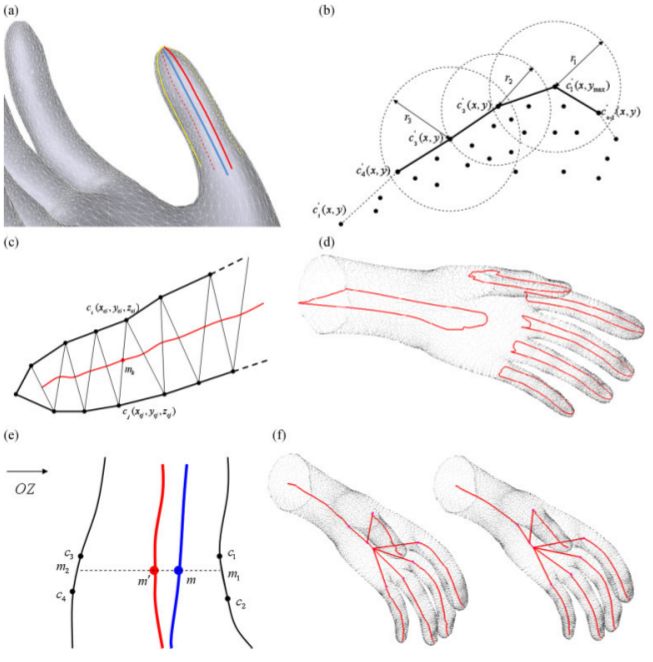
\includegraphics[width=.7\linewidth]{00_Rigging/Pictures/extraction_pic1.png}
	\caption[Schritte der Animation-Skelett-Extraktion]{ (a) 3D-Silhouetten (rot/gelb) und Mittelachse (blau), (b) Globale und Lokale Suche, (c) Findung der Mittelachse einer Silhouette (d) Zweite Silhouetten f�r die einzelnen Bereiche der Hand, (e) Begradigung der Mittelachse, (f) Vergleich des Kurven-Skeletts vor und nach der Mittelachsenbegradigung. Entnommen aus \cite{extraction}}
	\label{extraction_fig1}
\end{figure}


\subsection{Skelett-Einbindung}
\label{sec:skeleton-embedding}

Der nachfolgende Absatz behandelt das Thema der \nameref{sec:skeleton-embedding} welches sich auf die Ausarbeitung von Ilya Baran und Jovan Popovic \cite{embedding} st�tzt.

F�r diese Rigging-Methode ben�tigt man ein vorgefertigtes Animations-Skelett sowie ein Mesh. Um dieses Skelett bestm�glich in dem Modell zu platzieren, muss man ein Graph-Optimierungs-Problem l�sen. Um die Optimierung zu vereinfachen, wird das Volumen in mehreren Schritten reduziert. Am Ende erhalten wir einen Graphen, auf welchen unser vorgefertigtes Animations-Skelett gemapped werden kann.
In Abbildung \ref{embedding_fig1} ist das Verfahren vereinfacht graphisch dargestellt.
\begin{figure}[t]
	\centering
	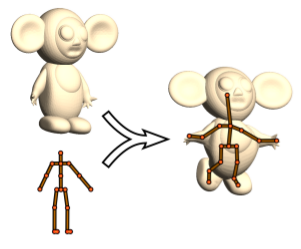
\includegraphics[]{00_Rigging/Pictures/embedding_pic1.png}
	\caption[Vereinfachte Darstellung der Skelett-Einbindung]{Vereinfachte Darstellung der Skelett-Einbindung. Entnommen aus \cite{embedding}}
	\label{embedding_fig1}
\end{figure}

\begin{figure}[t]
	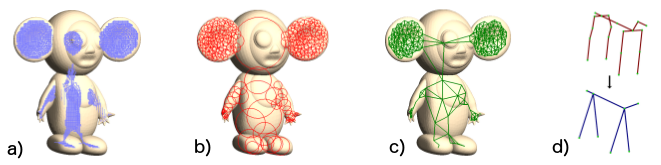
\includegraphics[width=\linewidth]{00_Rigging/Pictures/embedding_pic2.png}
	\caption[Schrittweise Darstellung wie ein Graph im Modell gefunden wird]{ a) Mediale Fl�chen b) Dichteste Kugelpackung c) Erzeugter Graph d) Original und vereinfachtes Skelett. Entnommen aus \cite{embedding}}
	\label{embedding_fig2}
\end{figure}

\subsubsection{Volumenreduktion}
\paragraph{Mediale Fl�chen}
\label{sec:medial_surface}
Der erste Schritt zur Volumenreduzierung ist das Finden der medialen Fl�chen. Diese sind ein �quivalent der Mittelachse von zweidimensionalen Fl�chen im dreidimensionalen Raum. Ein Punkt liegt auf dieser Fl�che, wenn er mehr als eine minimale Distanz von sich zur K�rperoberfl�che besitzt.
Man erwartet dass das eingebettete Skelett auf dieser Fl�che zu finden ist. In Abbildung \ref{embedding_fig2} a) sind diese medialen Fl�chen eines Meshs zu sehen.

\paragraph{Dichteste Kugelpackung}
\label{sec:sphere_packing}
Um das Volumen weiter zu reduzieren wird ein Graph erstellt, welcher die Gelenke als Knoten und die Knochen als Kanten hat. Um diesen Graph zu erzeugen wird eine Methode �hnlich der Methode zur Findung der \enquote{Dichtesten Kugelpackung}\footnote{\label{foot:1} Bei dieser Methode wird versucht Kugeln mit dem gleichen Radius in einem dreidimensionalen K�rper zu platzieren	, wobei die Kugeln sich nur ber�hren, aber nicht �berlappen d�rfen. Ziel dieses Verfahrens ist es, einen m�glichst minimalen Freiraum zwischen den Kugeln zu finden.} verwendet. Jedoch d�rfen sich bei dieser Methode die Kugeln �berlappen.

Jeder Punkt auf der medialen Fl�che dient als Mittelpunkt einer Kugel und hat als Radius seine Distanz zur Oberfl�sche des Meshs. Als Startpunkt wird der Punkt genommen, dessen Distanz zur Oberfl�che am gr��ten ist. Es d�rfen nur Kugeln hinzugef�gt werden, welche nicht den Mittelpunkt einer anderen Kugel umschlie�en. 

\subsubsection{Graph-Erzeugung}
\label{sec:graph_generating}
Anhand der erzeugten Kugeln, wird nun der Graph abgeleitet. Jeder Mittelpunkt ist ein Knoten im Graph. Sich schneidenden Kugeln oder Gabriel-Nachbarn (Erkl�rung: Abbildung \ref{gabriel}) repr�sentieren die Kanten im Graph. Jeder der erzeugten Knoten ist ein potenzieller Knoten und jede Kante ist eine potenzielle Verbindung (Knochen) im Skelett.

\begin{figure}[t]
	\centering
	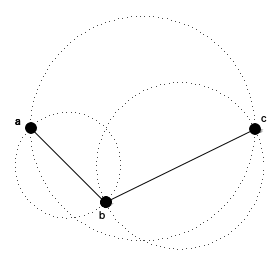
\includegraphics[]{00_Rigging/Pictures/gabriel.png}
		\caption[Erkl�rung von Gabriel-Nachbarn]{ links) $a$, $b$ und $b$, $c$ sind Gabriel-Nachbarn. Die Punkte $a$ und $c$ jedoch nicht. Da der Kreis mit dem Durchmesser $\overline{ac}$ den Punkt $b$ beinhaltet. Nachempfunden aus \cite{gabriel_neighbor}}
		\label{gabriel}
\end{figure}

\subsubsection{Kontinuierliche Optimierung der Skelett-Einbindung}
\label{optimal_skeleton_embetting}
Um das vorgegebene Skelett nun in das Modell einzubinden, wird der erzeugte Graph ben�tigt. Der erste Schritt hierbei ist es das vorgegebene Skelett zu vereinfachen. Das Original-Skelett hat $s$ Gelenke das reduzierte Skelett $r$ Gelenke. 
Es k�nnen alle Gelenke zweiten Grades (Knie, Elebogen, ...) reduziert werden. Diese Reduktion der Gelenke wird ben�tigt um die Freiheitsgrade der Straffunktionen (penalty functions) zu reduzieren.

Die Straffunktionen haben gro�en Einfluss auf die Qualit�t des Ergebnisses und der Selbst�ndigkeit des gesamten Verfahrens. Sie sind daf�r da, um ungeeignete Skelett-Einbindungen zu verhindern. Als ungeeignete M�glichkeiten k�nnen folgende Einbettungen betrachtet werden:
\begin{itemize}
	\item kurze Knochen
	\item unm�gliche Gelenkstellungen
	\item unterschiedliche Knochenl�ngen bei symmetrisch gekennzeichneten Knochen
	\item Gelenke welche als F��e markiert wurden sind nicht in Bodenn�he
	\item Knochenstr�nge mit der L�nge 0
	\item unm�gliche Knochenausrichtungen
	\item Gelenke, welche im Graph nah beieinander im originalem Skelett jedoch weit entfernt liegen
\end{itemize}
Um das optimale Gewicht f�r jede dieser Straffunktionen zu finden, wurde mit Hilfe einer St�tzvektormaschine versucht ein maximaler Breiter-Rand-Klassifikator (\enquote{margin linear classifier}) zu finden. Dieser Klassifikator versucht den Abstand zwischen der besten \enquote{schlechten} und der schlechtesten \enquote{guten} Einbettung zu maximieren.
\begin{equation}
\label{weight}
c = \min_{i=1}^{n}\vec{\Gamma}^T \vec{q_{i}} - \min_{i=1}^{m}\vec{\Gamma}^T \vec{p_{i}}
\end{equation}
$\vec{p}$ (\enquote{gut}) und $\vec{q}$ (\enquote{schlecht}) sind Vektoren welche die Einbettungen rep�sentieren. Der Vektor $\vec{\Gamma}$ enth�lt das Gewicht, $n$ und $m$ stehen f�r die Anzahl der \enquote{guten} bzw. \enquote{schlechten} Einbettungen. Idealerweise sollte $\vec{\Gamma}$ so gew�hlt werden, das $c$ gegen $1$ geht. 

Um die beste Einbettung zu finden wird Schritt f�r Schritt vorgegangen. Es wird an einem Punkt gestartet und die beste partielle Einbettung zum n�chsten Gelenk gesucht. Dies geschieht so lange, bis das komplette Skelett eingebunden ist.

Zum Schluss wird das ganze Skelett noch einmal optimiert, sprich die wegreduzierten Gelenke aus dem Original-Skelett werden wieder eingebunden, Knochenproportionen werden  hergestellt. Abbildung \ref{embedding_fig3} zeigt diese Optimierung. Dies geschieht �hnlich wie das Einbinden des Skeletts mit Straffunktionen. Diese Funktionen sind dieses Mal jedoch anders definiert. 

\begin{figure}[t]
	\centering
	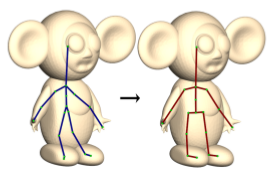
\includegraphics[]{00_Rigging/Pictures/embedding_pic3.png}
	\caption[Vergleich: Eingebundenes Skelett vor und nach der Optimierung]{Eingebundenes Skelett vor (blau) und nach (rot) der Optimierung. Entnommen aus \cite{embedding}}
	\label{embedding_fig3}
\end{figure}

\subsubsection{Zusammenfassung}
\label{sec:conclusion_embedding}
Analog zum Abschnitt \ref{conclusion_extraction} wird diese Rigging-Methode anhand der 3 Kenngr��en evaluiert.
Der von Baran und Popovic vorgestellte Algorithmus f�llt unter die Komplexit�t von $O(N^2)$, sie geben an, dass sie 16 verschiedene Modelle getestet haben. Die Modelle konnten in einer Zeit zwischen 12.6 und 77.1 Sekunden gerigged werden.

Bei der Allgemeing�ltigkeit ist der Algorithmus stark auf das vorgegebene Skelett eingeschr�nkt, im Beispiel \cite{embedding} auf humanoide Modelle. Ein weiterer Nachteil ist ebenfalls das kleine Modelle mit vielen kleinen Knochen generell (z.B. Schlangen) zu Problemen f�hren. Da diese durch die Straffunktionen ausgeschlossen werden. 
Von den 16 getesteten Modellen, siehe Abbildung \ref{embedding_fig4} wurden die meisten korrekt gerigged. Nur bei Modell 7, 10 und 13 kam es zu Problemen, diese konnten jedoch durch kleine Hinweise f�r die korrekte Gelenkplazierung durch den Benutzer gel�st werden.

Die Selbst�ndigkeit ist stark eingeschr�nkt durch die Pose des Modells. Diese muss sich m�glichst an dem Skelett orientieren, sonst w�rden die Straffunktionen daf�r sorgen, dass die Einbindungen wegen der Gelenk- und Knochenstellungen als \enquote{schlecht} markiert werden. Au�erdem erwartet der Algorithmus, dass das Modell mit beiden F��en am Boden steht.
\begin{figure}[t]
	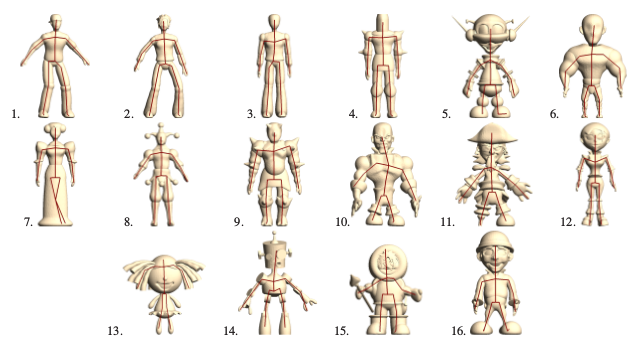
\includegraphics[]{00_Rigging/Pictures/embedding_pic4.png}
	\caption[Ergebnisse der Skelett-Einbindung]{Ergebnisse der Skelett-Einbindung. Entnommen aus \cite{embedding}}
	\label{embedding_fig4}
\end{figure}


	\section{Skinning}
\subsection{Was ist Skinning?}
{ %öffnende Klammer für hintergrundbild lokal
	\usebackgroundtemplate{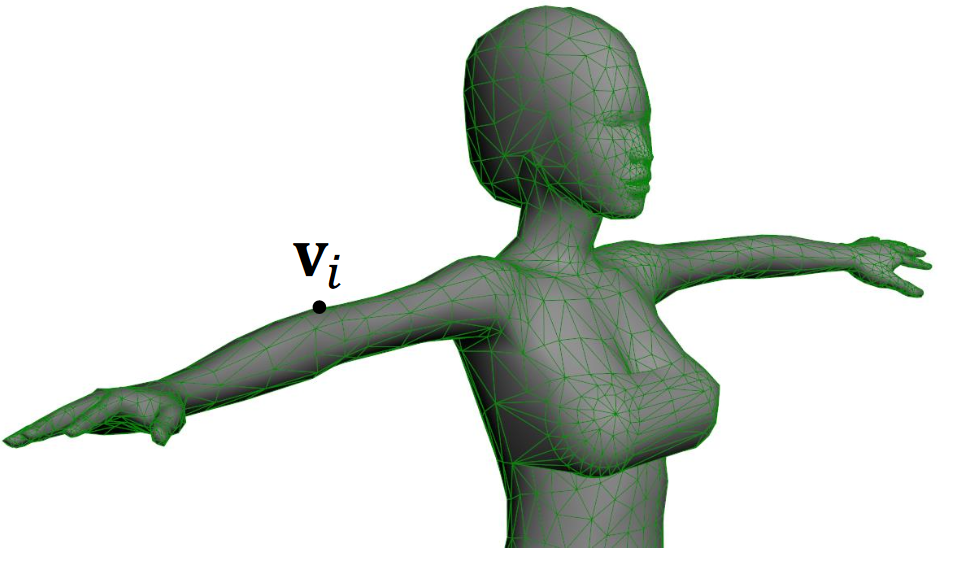
\includegraphics[width=\paperwidth,height=\paperheight]{01_Skinning/Pictures/SkinningIntro.PNG}}
	\begin{frame}{\Huge{Was ist Skinning?}}
		\blfootnote{Bildquelle: \cite{skinningcourse:2014}}
		
		\pdfnote{Frage an alle: Was soll jetzt mit dem geriggten Modell passieren}
		\pdfnote{Frage an alle: Welcher Ansatz wäre hier der Intuitive}

		
	\end{frame}
} %schließende klammer für hintergrundbild lokal

{

	\begin{frame}{\Huge{Transformationen}}

			
			\begin{figure}
				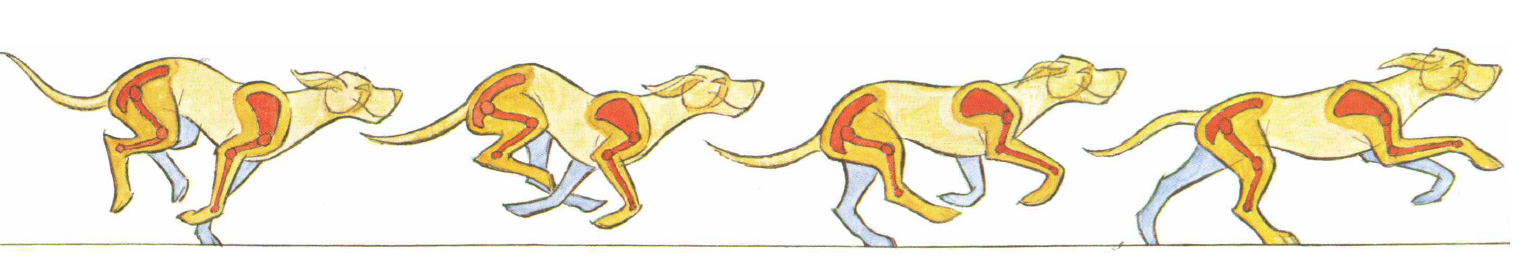
\includegraphics[width=1.0\textwidth]{01_Skinning/Pictures/Transformation.PNG}
			\end{figure}
		
		\blfootnote{Bildquelle: \cite{skinningcourse:2014}}
		
		\pdfnote{Offene Frage: Was heisst Transformation genau, wie kann man sie darstellen, was ist besonders und wichtig daran?}
		
	\end{frame}
}

{
	
	\begin{frame}{\Huge{Translation}}
		
		\begin{figure}
			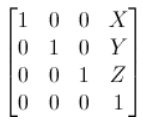
\includegraphics[width=0.3\textwidth]{01_Skinning/Pictures/Translation.PNG}
		\end{figure}
		
		
		\pdfnote{multiplikation zeigen}
		
	\end{frame}
}


{
	
	\begin{frame}{\Huge{Scale}}
		
		\begin{figure}
			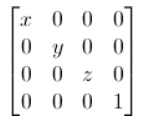
\includegraphics[width=0.3\textwidth]{01_Skinning/Pictures/scale.PNG}
		\end{figure}
		
		
		
		\pdfnote{multiplikation zeigen}
		
	\end{frame}
}

{
	
	\begin{frame}{\Huge{Rotation}}
		
		\begin{figure}
			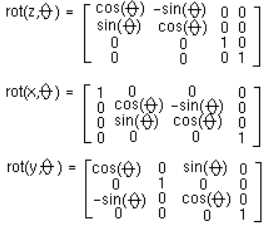
\includegraphics[width=0.6\textwidth]{01_Skinning/Pictures/rotation.PNG}
		\end{figure}
		
		
		\pdfnote{multiplikation zeigen}
		
	\end{frame}
}

{ %öffnende Klammer für hintergrundbild lokal
	\usebackgroundtemplate{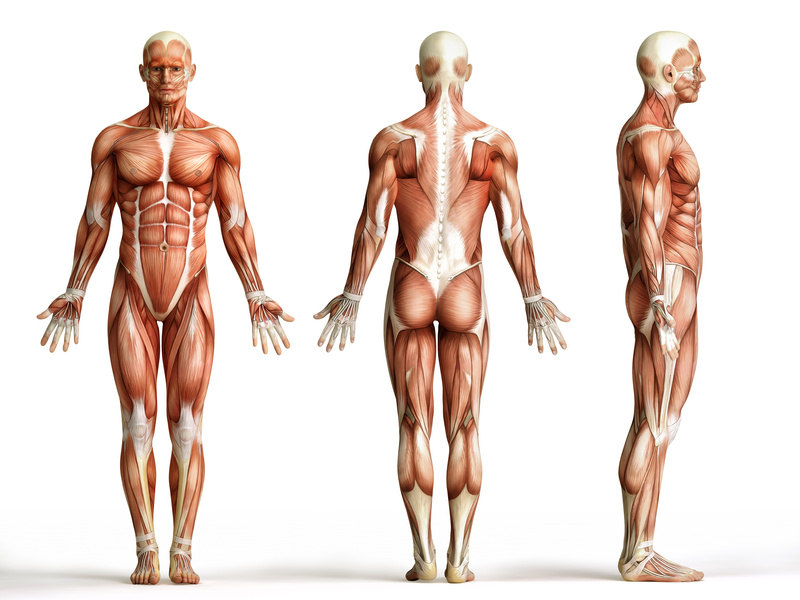
\includegraphics[width=\paperwidth,height=\paperheight]{01_Skinning/Pictures/physiologisch.jpg}}
	\begin{frame}{\Huge{Anatomische Modellierung}}
		\blfootnote{\colorbox{black!10}{Bildquelle: \cite{muskeln}}}
		
		\pdfnote{Aufbau des Menschen abbilden -> Daraus ergibt sich Realität}
		
		
		
	\end{frame}
} %schließende klammer für hintergrundbild lokal

{
	
	\begin{frame}{\Huge{Motion Capture}}
		
		\begin{figure}
			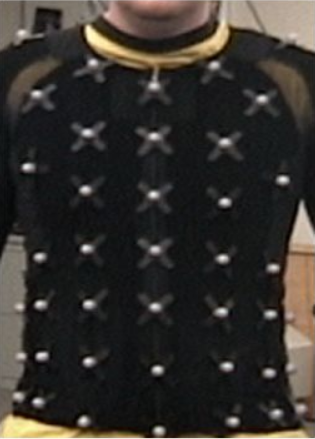
\includegraphics[width=0.4\textwidth]{01_Skinning/Pictures/breathing.PNG}
		\end{figure}
		
			\blfootnote{Bildquelle: \cite{dilorenzo2008breathing}}
		
		\pdfnote{Beobachting menschlicher Funktion}
		
	\end{frame}
}

	\begin{frame}{\Huge{Multipler Input}}

		
		\begin{figure}
			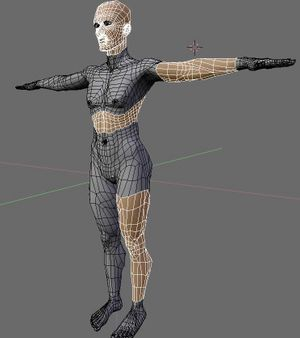
\includegraphics[width=0.5\textwidth]{01_Skinning/Pictures/multi.jpg}
		\end{figure}
		
		\blfootnote{Bildquelle: \cite{multi}}
		
		\pdfnote{Viel Input}
		
	\end{frame}


{ %öffnende Klammer für hintergrundbild lokal
	\usebackgroundtemplate{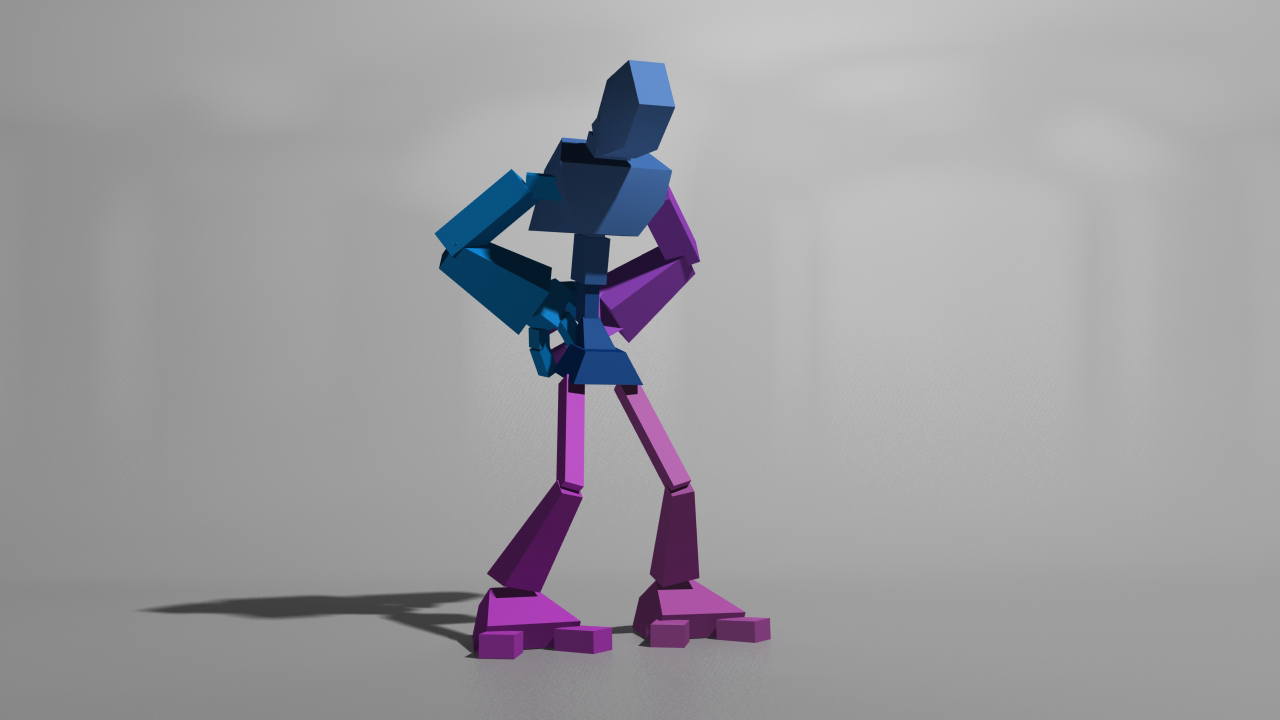
\includegraphics[width=\paperwidth,height=\paperheight]{01_Skinning/Pictures/geometrisch.jpg}}
	\begin{frame}{\colorbox{black!10}{\Huge{Geometrisches Skinning}}}
		\blfootnote{\colorbox{black!10}{Bildquelle: \cite{geo}}}
		
		\pdfnote{Knoten an Knochen}
		
		
		
	\end{frame}
} %schließende klammer für hintergrundbild lokal
\subsection{Lineares Modell}

	\begin{frame}{\Huge{Linear Skinning}}
		
		$$v'=W_{i}(v)$$
		
		\pdfnote{Lineares Modell erklären}
		
	\end{frame}

{ %öffnende Klammer für hintergrundbild lokal
	\usebackgroundtemplate{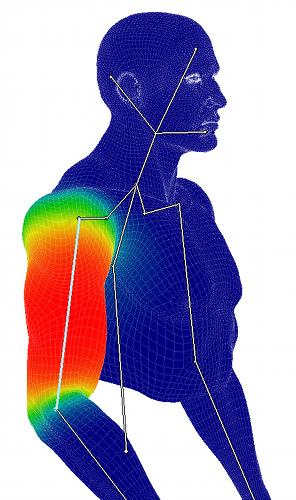
\includegraphics[width=\paperwidth,height=\paperheight]{01_Skinning/Pictures/weight.png}}
	\begin{frame}{\Huge{Weights}}
		\blfootnote{\colorbox{black!10}{Bildquelle: \cite{weights}}}
		
		\pdfnote{Abhängigkeit vom Knochen}
		
		
		
	\end{frame}
} %schließende klammer für hintergrundbild lokal

	\begin{frame}{\Huge{Heat Equilibrium}}
		
		\begin{figure}
			
\includegraphics[width=0.6\textwidth]{01_Skinning/Pictures/heat.png}
		\end{figure}
		
		\blfootnote{Bildquelle: \cite{heat}}
		
		\pdfnote{Aufteilung anhand von Hitze}
		
	\end{frame}
	
	\begin{frame}{\Huge{Linear Blend Skinning}}
		
		$$v'=\sum_{i=1}^{N}w_{i}W_{ji}(v)$$
		
		\pdfnote{Lineares Blend Skinning Modell erklären}
		
	\end{frame}
	
		\begin{frame}{\Huge{Linear Blend Skinning Matrix}}
			
			\begin{figure}
				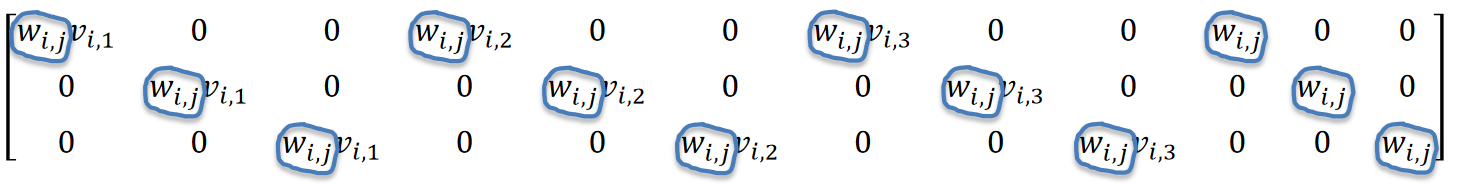
\includegraphics[width=1.0\textwidth]{01_Skinning/Pictures/lbsmatrix.png}
			\end{figure}
			
			\blfootnote{Bildquelle: \cite{skinningcourse:2014}}
			
			\pdfnote{LBS Matrix erklären}
			
		\end{frame}
		
		\begin{frame}{\Huge{Linear Blend Skinning Artefakte}}
			
			\begin{figure}
				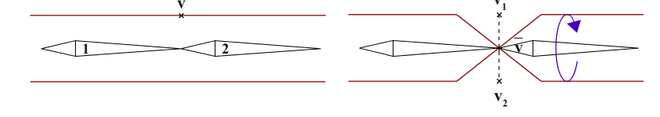
\includegraphics[width=1.2\textwidth]{01_Skinning/Pictures/rotationsartefakt.png}
			\end{figure}
			
			\blfootnote{Bildquelle: \cite{weights}}
			
			\pdfnote{Aufteilung anhand von Hitze}
			
		\end{frame}
		
				\begin{frame}{\Huge{Linear Blend Skinning Artefakte}}
					
					\begin{figure}
						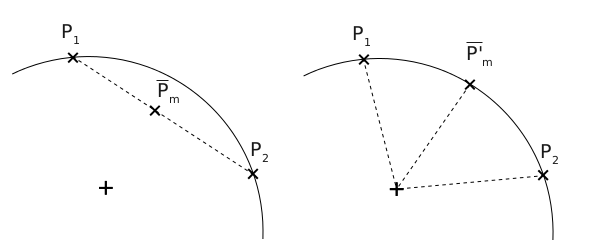
\includegraphics[width=0.6\textwidth]{01_Skinning/Pictures/interpolation_angle.png}
					\end{figure}
					
					\blfootnote{Bildquelle: \cite{weights}}
					
					\pdfnote{Aufteilung anhand von Hitze}
					
				\end{frame}

	\begin{frame}{\Huge{Facial Blend Skinning}}

		
		$$S=S0+\sum_{i}w_{i}(S_{i}-S_{0})$$
		
		\pdfnote{Lineares Blend Skinning Modell erklären}
		
	\end{frame}

				\begin{frame}{\Huge{Facial Blend Skinning}}
					
					\begin{figure}
						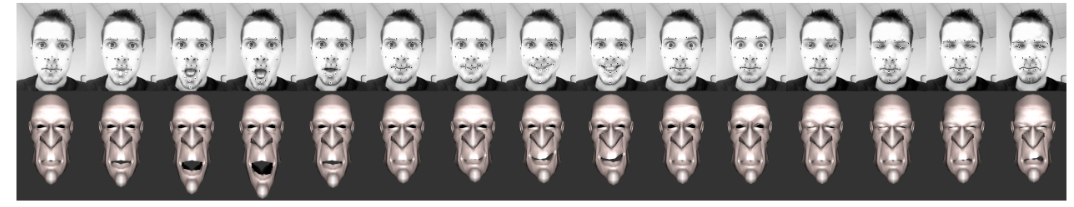
\includegraphics[width=1.2\textwidth]{01_Skinning/Pictures/face.png}
					\end{figure}
					
					\blfootnote{Bildquelle: \cite{dutreve2008feature}}
					
					\pdfnote{Aufteilung anhand von Hitze}
					
				\end{frame}

\subsection{Quaternionen}
				\begin{frame}{\Huge{Quaternionen}}

					\begin{figure}
						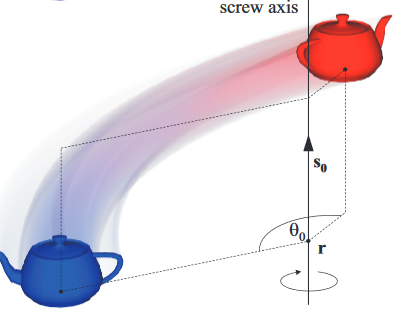
\includegraphics[width=0.5\textwidth]{01_Skinning/Pictures/Quaternionen.png}
					\end{figure}
					
					\blfootnote{Bildquelle: \cite{kavan2008geometric}}
					
					\pdfnote{Video 1}
					
				\end{frame}
				
		\begin{frame}{\Huge{Dual Quaternionen Skinning}}
			
			$$\mathbf{\dot q} =  \frac{\sum_{i=1}^n w_i \mathbf{\dot q}_i}{\| \sum_{i=1}^n w_i \mathbf{\dot q}_i \|}$$
			
			\pdfnote{Lineares Blend Skinning Modell erklären}
			
		\end{frame}
		
				\begin{frame}{\Huge{Linear Blend Skinning}}
					
					\begin{figure}
						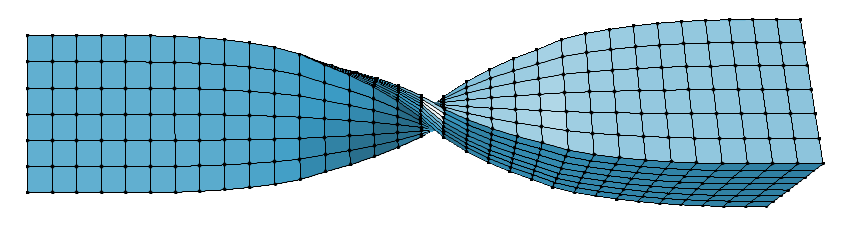
\includegraphics[width=1.0\textwidth]{01_Skinning/Pictures/lbsgrad.png}
					\end{figure}
					
					\blfootnote{Bildquelle: \cite{weights}}
					
					\pdfnote{Aufteilung anhand von Hitze}
					
				\end{frame}
				
						\begin{frame}{\Huge{Dual Quaternion Skinning}}
							
							\begin{figure}
								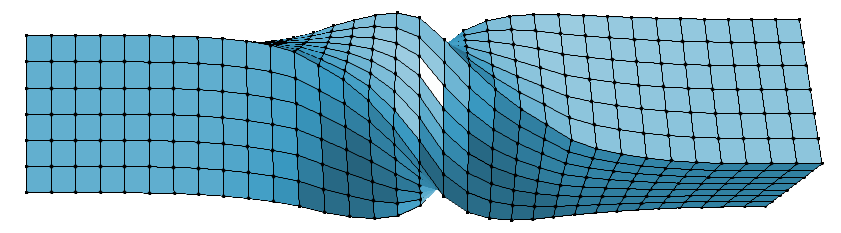
\includegraphics[width=1.0\textwidth]{01_Skinning/Pictures/dqsgrad.png}
							\end{figure}
							
							\blfootnote{Bildquelle: \cite{weights}}
							
							\pdfnote{Aufteilung anhand von Hitze}
							
						\end{frame}
						
				\begin{frame}{\Huge{Artefakte Dual Quaternionen}}
					
					\begin{figure}
						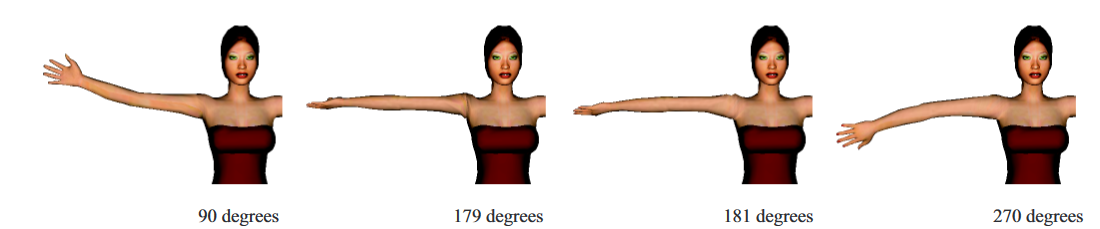
\includegraphics[width=1.0\textwidth]{01_Skinning/Pictures/dqsgradartefakte.png}
					\end{figure}
					
					\blfootnote{Bildquelle:\cite{kavan2008geometric}}
					
					\pdfnote{Video 1}
					
				\end{frame}
				
					\begin{frame}{\Huge{Fazit}}
							
							\begin{figure}
								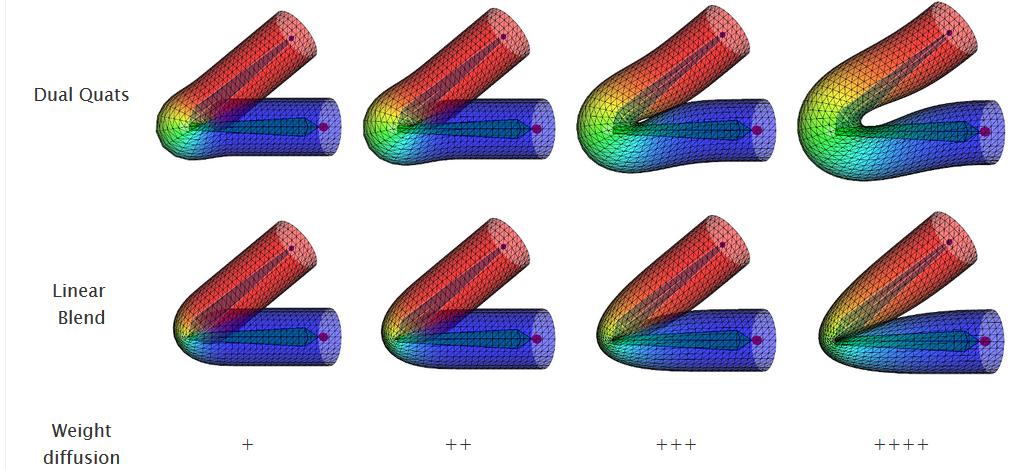
\includegraphics[width=0.8\textwidth]{01_Skinning/Pictures/lbsvsdqs.png}
							\end{figure}
							
							\blfootnote{Bildquelle: \cite{weights}}
							
							\pdfnote{Zusammenfassung, video 2}
					
						\end{frame}
		
	\section{Rendering im Film}
\subsection{Einleitung}
\label{sec:introduction}
Ist der Charakter korrekt geriggt und geskinnt muss er nun noch entsprechend seiner Eigenschaften korrekt gerendert werden. Rendering bezeichnet im Allgemeinen das Erstellen eines zweidimensionalen Bildes aus einer dreidimensionalen Szene oder eines Objektes unter Ber�cksichtigung physikalische Gr��en wie Licht, Schatten und Materialien \cite{renderingDefinition}. Dieser Prozess findet in einer Vielzahl von unterschiedlichen Bereichen Anwendungsf�lle. Zum einen in der Darstellung von Computerspielen, bei Konstruktionen in CAD-Programmen aber auch bei CGI in aktuellen Filmen. 
Jeder Anwendungsfall hat andere Anforderungen und Priorit�ten an das Rendering. W�hrend Computerspiele vor Allem ein schnelles Erzeugen von Bildern ben�tigen, kommt es in Filmen auf eine m�glichst reale und detailreiche Darstellung an. Das folgende Kapitel besch�ftigt sich mit den besonderen Anforderungen an das Rendering im Film. 

Hier m�ssen die Bilder in einer angemessenen Zeit gerendert werden und trotzdem einen hohen Detailgrad aufweisen. Zus�tzlich m�ssen sich Licht und Materialien im Filmkontext korrekt verhalten und dem Betrachter das Gef�hl einer realistischen Szene geben. Das hei�t es m�ssen Reflexionen, Brechungen von Licht, sowie Schatten und Materialeigenschaften wie Transparenz ber�cksichtigt werden. All das kann bereits bei relativ kleinen Objekten zu aufwendigen Berechnungen f�hren. Beim Film arbeiten wir jedoch mit sehr komplexen Szenen, welche aus vielen Objekten bestehen. Aus diesen Szenen m�ssen f�r eine Sekunde Film 24 hochaufl�sende Bilder erstellt werden. Im Folgenden werden zun�chst grundlegende Eigenschaften von Beleuchtung und Materialien er�rtert, um dann unter Ber�cksichtigung der oben genannten Anforderungen, auf die Erzeugung einer komplett synthetischen Szene wie in \ref{cars} als auch das Einf�gen unseres synthetischen Charakters in eine reale Szene einzugehen.

\begin{figure}[t]
	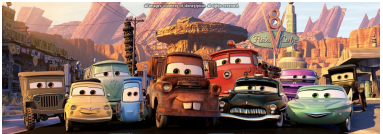
\includegraphics[width=13cm]{02_Rendering/img/cars.png}
	\caption[Bild aus dem Film Cars]{Bild aus dem Film Cars. Entnommen aus \cite{cars}}
	\label{cars}
\end{figure}

\subsection{Licht}
Jede Rendering Technik versucht das gleiche physikalische Ph�nomen abzubilden. N�mlich die Streuung von Licht \cite{renderingEquation}.
Dabei ist zu beachten, dass sowohl spekulare sowie diffuse Reflexionen auftreten k�nnen. Eine ideal spekulare Reflexion kommt vor wenn ein Lichtstrahl eine Spiegeloberfl�che trifft. Hier wird nur ein einziger Strahl nach dem Gesetz Einfallswinkel ist gleich Ausfallswinkel reflektiert. Ideal diffuse Reflexion tritt hingegen auf wenn ein Lichstrahl auf eine ideal matte Oberfl�che trifft und gleichm��ig in alle Richtungen gestreut wird. Wie viel Licht sich an einem Punkt im Raum befindet ergibt sich zum einen aus dem direkt von einer Lichtquelle einfallenden Licht, als auch durch das Licht, welches von umliegenden Punkten auf den Punkt reflektiert wird. Der Vorgang die passende Farbe entsprechend der Lichteinstrahlung und des Materials zu finden nennt sich Shading. Dieser Vorgang wird mit Hilfe lokaler Reflexionsmodelle beziehungsweise globaler Beleuchtungsmodelle angen�hert. Reale Bilder ben�tigen fast immer eine Kombination der beiden Modelle.

\subsubsection{Lokale Reflexionsmodelle}
\label{localLight}
In der Realit�t verhalten sich verschiedene Materialien bei gleicher Beleuchtung unterschiedlich bez�glich ihrer Reflexionseigenschaften. Die Menge des reflektierten Lichts eines Punktes bei direkter Beleuchtung in eine bestimmte Richtung kann mittels einer Bi-Directional Reflection Distribution Function (BRDF) berechnet werden. Hierbei wird der Punkt v�llig isoliert in der Szene betrachtet. Wechselwirkungen mit anderen Objekten wie Schatten oder gegenseitige Reflexionen werden im lokalen Model nicht ber�cksichtig.  Alan Watt beschreibt diese Funktion in seinem Buch 3D Computergrafik wie folgt \cite{localLightCite}:
\begin{equation}
\label{BRDFEq}
BRDF=f(\theta in, \phi in, \theta ref, \phi ref) = f(L, V)
\end{equation}
Dabei beschreiben $\phi in$ beziehungsweise $\phi ref$ den Einfallswinkel sowie $\theta in$ und $\theta ref$ den Brechungswinkel der Strahlen. Die aus \cite{localLightCite} entnommene Grafik \ref{BRDF} verdeutlicht die Beziehung der Parameter.
\begin{figure}[t]
	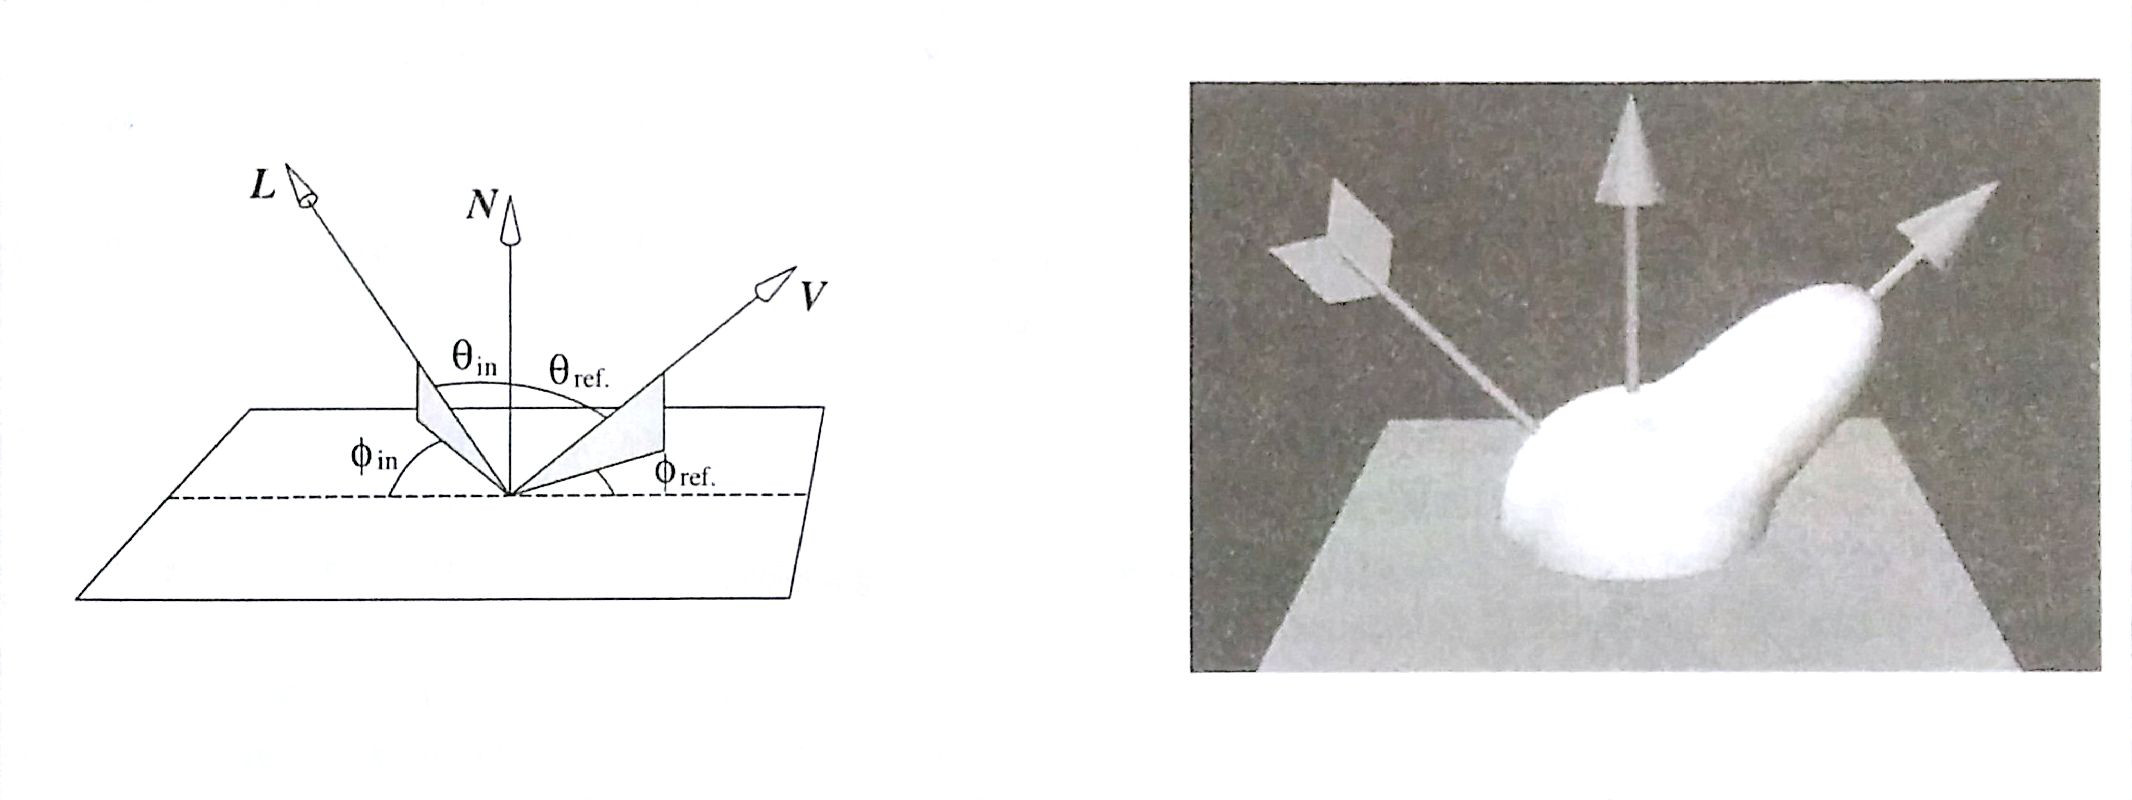
\includegraphics[width=13cm]{02_Rendering/img/brdf.jpg}
	\caption[BRDF]{BRDF zur Beschreibung des Verh�ltnisses des einfallenden Lichts $L$ und des reflektierten Lichts $V$}
	\label{BRDF}
\end{figure}
Um die unterschiedlichen Reflexionseigenschaften von Materialien zu simulieren werden verschiedene BRDFs modelliert. Die Kombination von einzelnen berechneten spekularen beziehungsweise diffusen Komponenten simuliert das Verhalten realer Oberfl�chen. Im Folgenden werden zwei Modelle zur Reflexion vorgestellt wie sie in \cite{brdf, brdf2} beschrieben sind.

\begin{itemize}
	\item \textbf{Lambertsche Reflexion.} Bei der Lambertschen Reflexion geht man davon aus, dass eine beleuchtete Oberfl�che bei gleicher Lichtintensit�t in jede Richtung mit der gleichen Intensit�t reflektiert. Sie ist damit gut zur Darstellung diffuser Reflexionen also matter Oberfl�chen wie Papier geeignet. Da die Lambertsche BRDF nur von der Intensit�t des einfallenden Lichts abh�ngt, kann sie ohne Ber�cksichtigung der Reflexionsrichtung berechnet werden. Die Intensit�t des reflektierten Lichts ergibt sich durch $I_{D} =\omega_{i} \cdot NCI_{L}$. Durch das Skalarprodukt von der Richtung des eintreffenden Lichtstrahls $\omega_{i}$ und der Normalen der Fl�che $N$ geht bei einem steil eintreffenden Lichtstrahl ein h�herer Wert der Farbe $C$ abh�ngig von der Lichtintensit�t $I_{L}$ in die Intensit�t des reflektierten Lichtstrahls $I_D$ ein. Ein mit einer Lambertschen BRDF erstelltes Dreieck ist in \ref{lambert} zu sehen.
	
	\item \textbf{Blinn-Phong Model.} Das Blinn-Phong Model basiert auf der Lambertschen Reflexion. Jedoch wird ein optisches Glanzlicht hinzugef�gt wenn die Normale der Fl�che etwa in der Mitte zwischen eingehenden und reflektierten Licht liegt. Es werden also diffuse und spekulare Reflexionen eingesetzt um zum Beispiel Metalle darzustellen. Die Blinn-Phong BRDF l�sst sich wie folgt berechnen:

\begin{eqnarray}
\label{blinnPhongEquation}
f_{s}(\omega_{i}, \omega_{o})=\frac{k_{L}}{\pi} + k_{G}\frac{8 + s}{8\pi}z^s
\end{eqnarray}
\begin{eqnarray*}
z=max(0,h \cdot n)
\end{eqnarray*}
\begin{eqnarray*}
h=\frac{\omega_{i} + \omega_o}{2}
\end{eqnarray*}



$h$ ist die Winkelhalbierende und befindet sich in der Mitte zwischen dem einfallenden Licht $\omega_i$ und der ausgehenden Reflexion $\omega_o$. Je kleiner der Winkel dieser Winkelhalbierenden und der Oberfl�chennormalen $n$ ist desto gr��er wird der Wert $z$. Je h�her $z$ desto st�rker geht die Glanzkonstante $k_G$ in die Formel ein. $k_G$ kontrolliert die Intensit�t und Farbe des optischen Glanzlichts. Analog dazu bestimmt Lambertsche Konstante $k_L$ die Intensit�t und Farbe der matten Stellen der Oberfl�che. Der Gl�ttegrad $s$ gibt an wie glatt die Oberfl�che ist. Dabei sind niedrige Werte um die 60 f�r Leder oder mattes Plastik und hohe Werte um die 2000 f�r stark spekulare Oberfl�chen wie zum Beispiel bei Autolacken oder Keramikoberfl�chen. Der Normalisierungsfaktor $\frac{8 + s}{8\pi}$ erh�ht die Intensit�t der Glanzlichter f�r glatte Oberfl�chen. Die 8ter entstehen durch die Rundung der Konstanten der L�sung des Integrals f�r den Glanzlichtterm �ber die gesamte Hemisph�re.
Ein mit der Blinn-Phong BRDF gerendertes Dreieck ist in Abbildung \ref{blinnPhong} zu sehen. 
\end{itemize}

\begin{figure}
\centering
\begin{subfigure}{.5\textwidth}
  \centering
  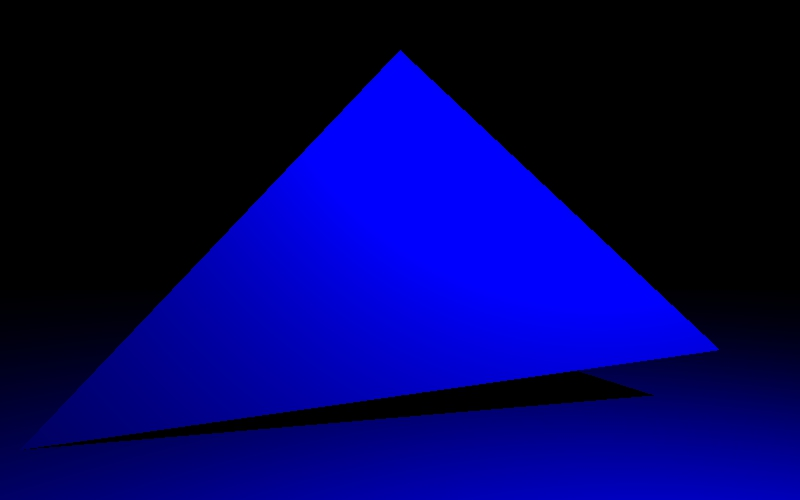
\includegraphics[width=.5\linewidth]{02_Rendering/img/lambertian.jpg}
  \caption[Lambertsches Dreieck]{Lambertsche BRDF}
  \label{lambert}
\end{subfigure}%
\begin{subfigure}{.5\textwidth}
  \centering
  
\includegraphics[width=.5\linewidth]{02_Rendering/img/glossy.jpg}
  \caption[Blinn-Phong Dreieck]{Blinn-Phong BRDF}
  \label{blinnPhong}
\end{subfigure}
\caption{Vergleich von Lambertschen BRDF und einer Blinn-Phong BRDF.}
\label{vergleich}
\end{figure}

\subsubsection{Globale Beleuchtungsmodelle}
Im Gegensatz zu den \nameref{localLight}n ber�cksichtigen globale Beleuchtungsmodelle nicht nur Licht welches direkt von einer Lichtquelle auf einen Punkt auftrifft sondern auch alles Licht welches �ber Reflexionen anderer Objekte verteilt wird. Um dies zu realisieren muss Licht durch die gesamte Szene hinweg verfolgt werden und nicht nur von der Lichtquelle zu einem Punkt und dann zum Betrachter. Es ist leicht ersichtlich, dass die Ber�cksichtigung globaler Reflexionseffekte eine deutlich h�here Komplexit�t als die Berechnung lokale Reflexionsmodelle aufwei�t. Einen mathematischen Ansatz zur Berechnung der Intensit�t der Beleuchtung an einem Punkt $x$ �ber einen anderen Punkt $x'$ ver�ffentlichte Kajiya 1986 in dem Paper \textit{The Rendering Equation}. Es handelt sich um eine v�llig allgemeine Aussage �ber das Problem der globalen Beleuchtung. Die Rendering Gleichung nach \cite{renderingEquation} ergibt sich aus:

\begin{equation}
\label{renderingEquation}
	L(x, x')=g(x, x') * \lbrack L_e(x,x') + \int_{s} p(x,x',x'')L(x',x'')dx''\rbrack
\end{equation}

Die Lichtintensit�t am Punkt $x$ ergibt sich aus dem Licht welches von $x'$ auf $x$ gestrahlt wird und dem Integral �ber alle Punkte aller Oberfl�chen der Szene $s$. $p(x,x' ,x'')$ nennt Kajiya den Drei-Punkt-Transport-Reflexionsgrad. Dieser entspricht den oben genannten BRDF welche die Reflexionseigenschaften f�r das Licht welches von $x''$ �ber $x'$ zu $x$ gelangt, beschreibt. W�hrend $L(x',x'')$ die Intensit�t des Lichts von Punkt $x''$ zu $x$ angibt. Der geometrische Term $g(x,x')$ dient der Berechnung der Sichtbarkeit der beiden Punkte und kann Werte zwischen $0$ wenn die Punkte sich gar nicht sehen und $1$ wenn eine optimale Sichtbarkeit vorliegt annehmen.
Mit Hilfe der Rendering Gleichung kann also theoretisch die globale Beleuchtung eines jeden Punktes abh�ngig von allen anderen Punkten berechnet werden. Dabei handelt es sich um ein blickwinkelunabh�ngiges Ergebnis. Das hei�t die Werte werden ohne Ber�cksichtigung der Position des Betrachters berechnet. Leider ist das Integral der Rendering Gleichung so komplex, dass es analytisch nicht berechnet werden kann. Es gibt aber Algorithmen welche die Komplexit�t reduzieren und Ergebnisse liefern, welche sich an die Rendering Gleichung ann�hern.

\subsection{Rendering Techniken}
Wie bereits erw�hnt ist die Rendering Gleichung analytisch nicht berechenbar. Da jedoch in der Realit�t diffuse Reflexionen einen gro�teil der Beleuchtung einer Szene ausmachen, kann die globale Beleuchtung im Rendering nicht vernachl�ssigt werden. Gerade im Film wird sie zur realistischen Darstellung von Objekten ben�tigt. Desweiteren muss eine professionelle Rendering Technik noch einige weitere F�higkeiten mitbringen. Catmull, Cook und Carpenter beschreiben diese in ihrem Paper zum Pixar eigenen Renderer Reyes wie folgt \cite{REYES}:

\begin{itemize}
	\item \textbf{Model Komplexit�t.} In einem mit CGI versehenen Film sollen Bilder erzeugt werden, welche visuell besonders ansprechend und detailreich sind. Das setzt voraus, dass Szenen mit einer Vielzahl von einzelnen Objekten die wiederum unterteilt sein k�nnen gerendert werden k�nnen.
	
	\item \textbf{Model Unterschiedlichkeit.} Die verwendete Rendering Technik muss eine Vielzahl von geometrischen Primitiven verarbeiten k�nnen. Sowohl Dreiecke, Vierecke als auch Partikel Systeme.
	
	\item \textbf{Komplexes Shading.} Die Reflexionseigenschaften verschiedener Materialien und Oberfl�chen sind �u�ert unterschiedlich und komplex. Eine gute Rendering Technik gibt dem Anwender die M�glichkeit selbst einen Shader zu implementieren. Dabei muss es auch m�glich sein Textur- oder Umgebungs-Maps einzusetzen.
	
	\item \textbf{Geschwindigkeit.} Um einem Film mit einer L�nge von zwei Stunden und 24 Bildern pro Sekunde in einem Jahr zu rendern wird eine Rendering Dauer von 3 Minuten pro Bild ben�tigt. Rendering Farms und verteiltes Rendering erm�glichen ein schnelleres Erstellen synthetischer Bilder, trotzdem muss eine professionelle Rendering Technik gerade f�r komplexe Szenen hoch performant funktionieren.
	
	\item \textbf{Bild Qualit�t.} Die gerenderten Bilder d�rfen keine Treppen-  oder Facettenartefakte aufweisen.
	
	\item \textbf{Flexibilit�t.} Im Laufe der Zeit werden immer neue und bessere Rendering Techniken entwickelt werden. Eine aktuelle Rendering Technik sollte flexibel genug sein neue Methodiken in den bestehenden Rendering Prozess zu integrieren.
\end{itemize}

Im Folgenden werden zwei Rendering Techniken besprochen, welche eine Ann�herung an die durch die Rendering Gleichung beschriebene Globale Beleuchtung erm�glichen und die oben genannten Anforderungen erf�llen. Die Techniken werden bereits zur Erzegung synthetischer Filme eingesetzt und werden in den von Pixar Animation Studios bereit gestellten Paper \cite{cars} und \cite{REYES} beschrieben.

	
	\bibliography{RSR}
	
\end{document}
